
% vim: set ts=4 sw=4 tw=80 noexpandtab:
%******************************************************************************%
%                                                                              %
%                   Machine_Learning_02.tex                                    %
%                   Made by: ikourkji                                          %
%                                                                              %
%******************************************************************************%

\documentclass{42-en}

%******************************************************************************%
%                                                                              %
%                                   Prologue                                   %
%                                                                              %
%******************************************************************************%

\begin{document}

\title{Introduction to Machine Learning}
\subtitle{Linear Regression}

\member {Jeson}{ljunzhen@42.us.org}
\member {}{Jesonleejunzhen.com}

\summary
{
Intro to types of machine learning and data pre-processing 
}

\maketitle

\tableofcontents

%Initialisation des headers d'exercices

\newpage

\bigskip

\centerline{
\includegraphics[width=150mm]{images/dontpanic.png}}

\centerline{\texttt{Eat, Sleep, Code, Repeat.}}

%******************************************************************************%
%                                                                              %
%                           Welcome to the World of AI                         %
%                                                                              %
%******************************************************************************%

\chapter{Welcome to the World of AI}

\centerline{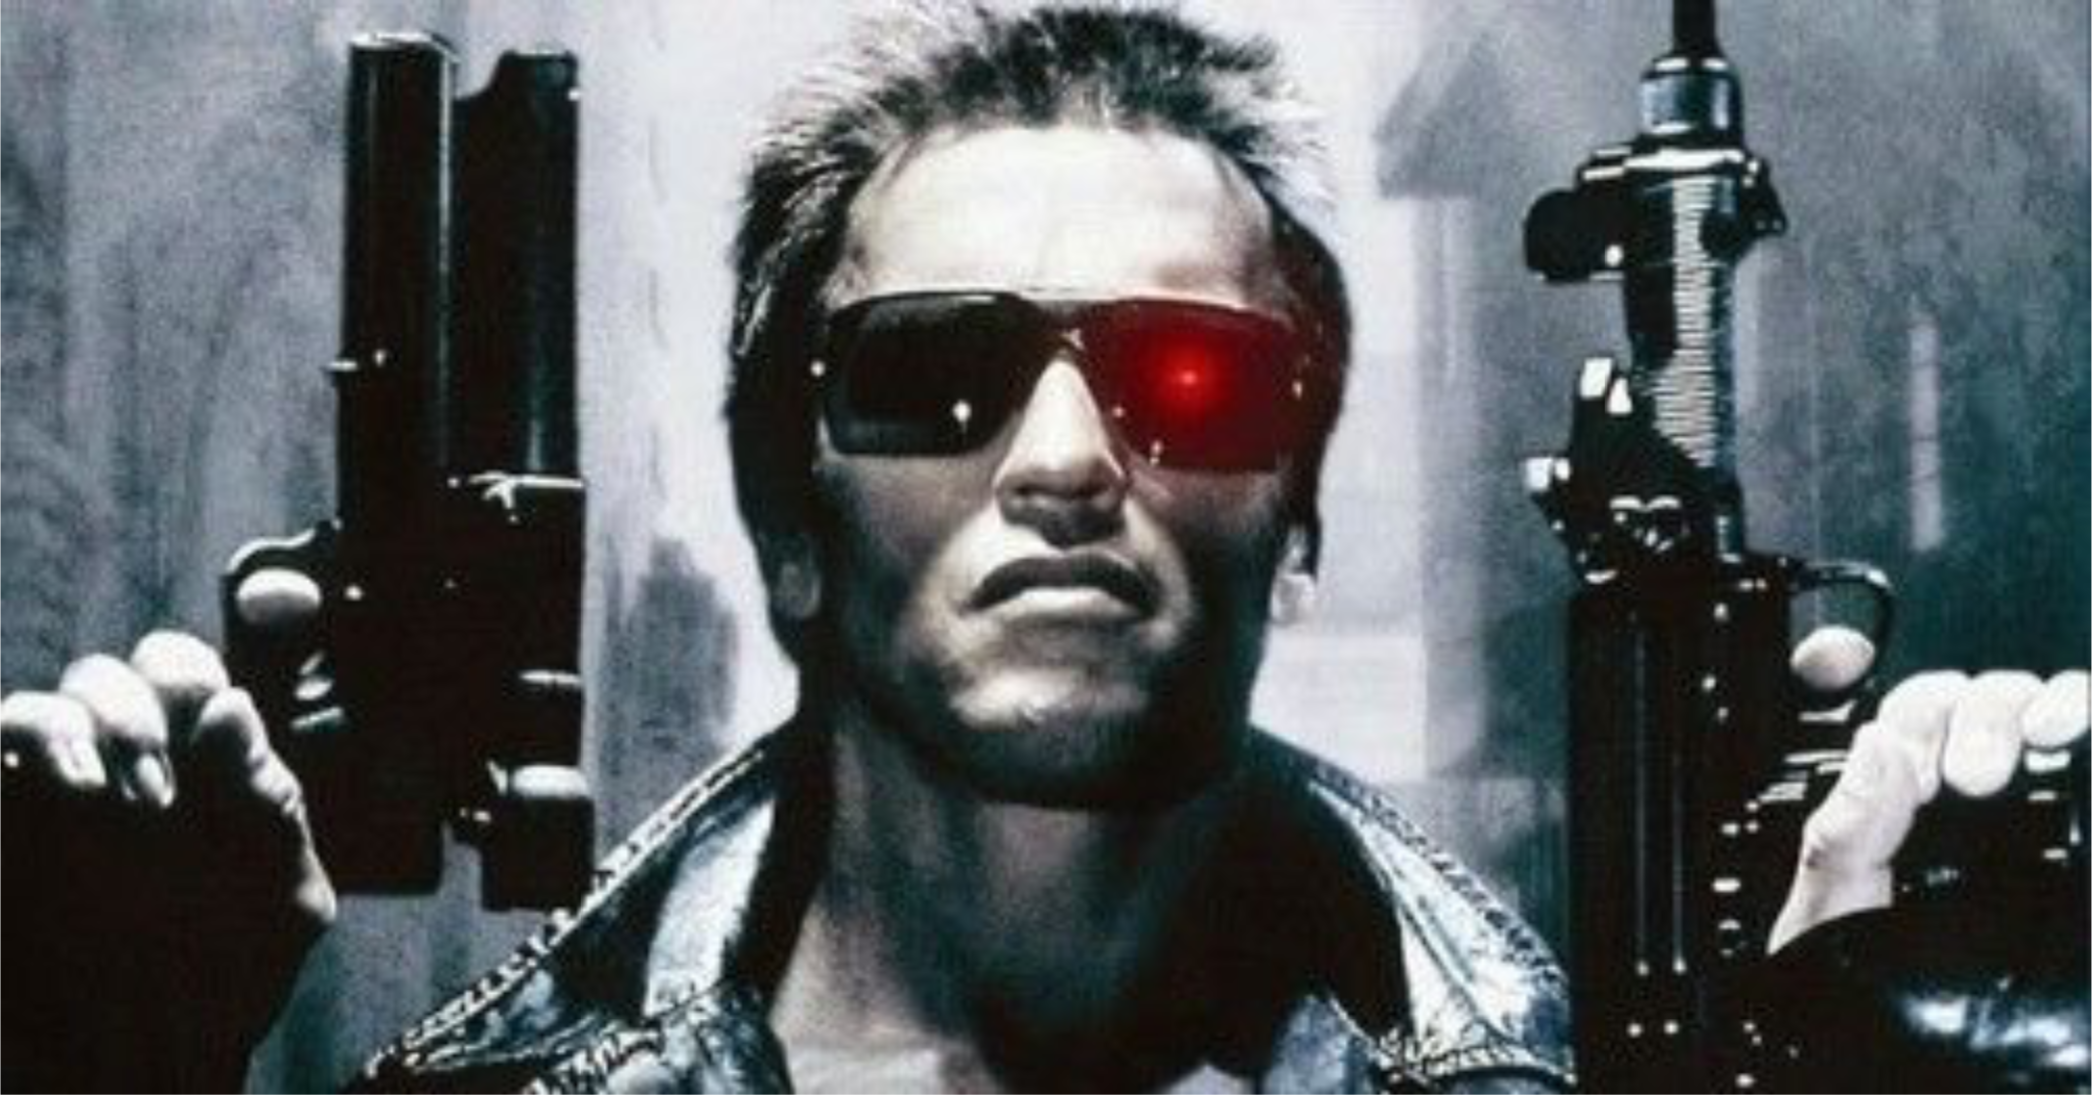
\includegraphics[width=150mm]{images/ahnold.png}}

\section*{Okay... So what the heck is A.I. all about?}

Artificial Intelligence is not some magical program that can think like a human. The mechanism behind it is to utilize different mathematical algorithms to learn from a tremendous amount of structured data to solve dedicated cognitive problems that originally could only be solved by human intelligence. The robust part of A.I. is it can acquire a pattern from the provided data to solve a problem in high accuracy.\\
  
TL;DR - A.I. learns from the data fed \textbf{to it} by a human to solve a dedicated problem.\\

\centerline{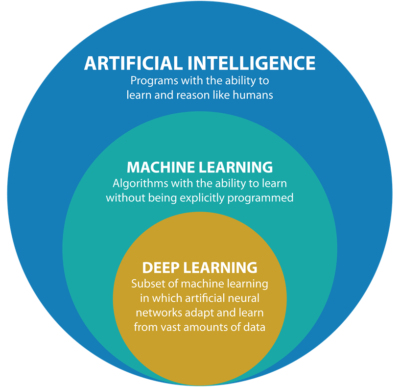
\includegraphics[width=100mm]{images/learning_diag.png}}

\section*{What is Machine Learning?}

Machine Learning (ML) is defined as the use of algorithms and computational statistics to learn from data without being explicitly programmed. It is a subsection of the artificial intelligence domain within computer science.\\

There some variations of how to define the types of Machine Learning Algorithms but commonly they can be divided into categories according to their purpose and the main categories are the following:\\
\begin{itemize}
    \item Supervised learning
    \item Unsupervised learning
    \item Reinforcement learning
\end{itemize}
Let’s look at each type in detail.

\newpage

\section*{Supervised Learning}

\centerline{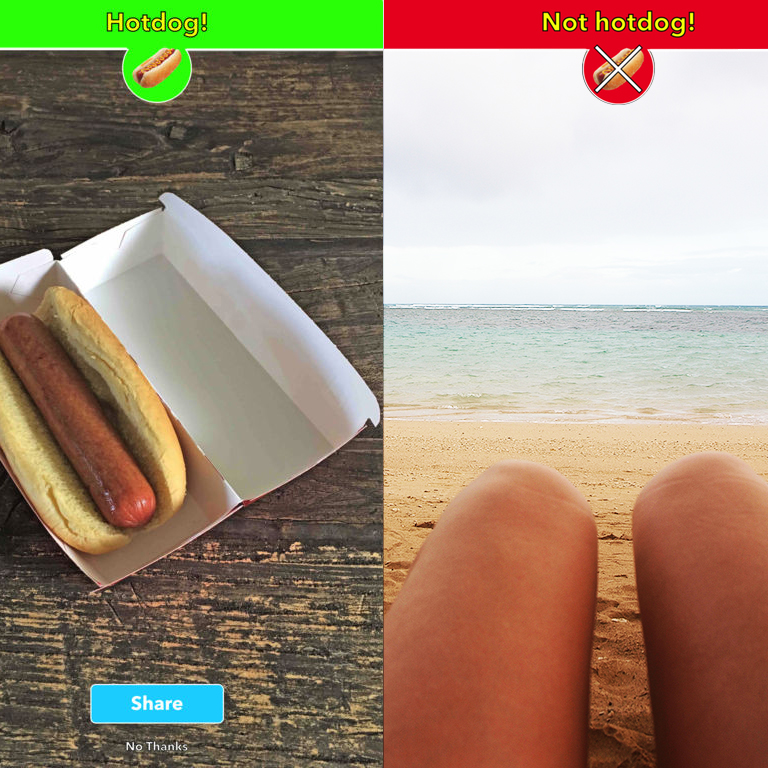
\includegraphics[width=75mm]{images/hotdogs_legs.jpg}}

In supervised learning, we are given a data set and already know what our correct output should look like, having the idea that there is a relationship between the input and the output.\\

The system tries to learn from the previous examples that are given. Supervised Learning is called supervised because the data scientist acts as a guide to teach the algorithm what conclusions it should come up with. It’s similar to the way a child might learn arithmetic from a teacher. Supervised learning requires that the algorithm’s possible outputs already be known and that the data used to train the algorithm is already labeled with correct answers. For example, a classification algorithm will learn to identify animals after being trained on a dataset of images that are properly labeled with the species of the animal and some identifying characteristics.\\

Supervised learning problems are categorized into "regression" and "classification" problems. In regression problems, we are trying to predict results within a continuous output, which means we are trying to map input variables to some continuous function. In a classification problem however, we are predicting results in a discrete output. In other words, we are trying to map input variables into discrete categories such as “yellow” and “not yellow”.\\

\hint{Google regression and classification to learn more.}\\

The mapping function is expressed as Y = f(X).\\

\centerline{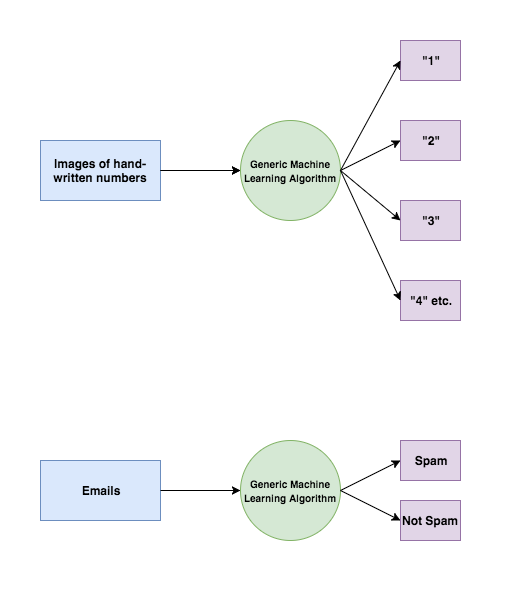
\includegraphics[width=125mm]{images/sort_chart.png}}

Examples of supervised learning:\\
\textbf{Face detection:} Identify faces in images (or indicate if a face is present).\\
\textbf{Email filtering:} Classify emails into spam and not-spam.\\
\textbf{Medical diagnosis:} Diagnose a patient as a sufferer or non-sufferer of some disease.\\
\textbf{Weather prediction:} Predict, for instance, whether or not it will rain tomorrow.\\

\section*{Unsupervised Learning}

\centerline{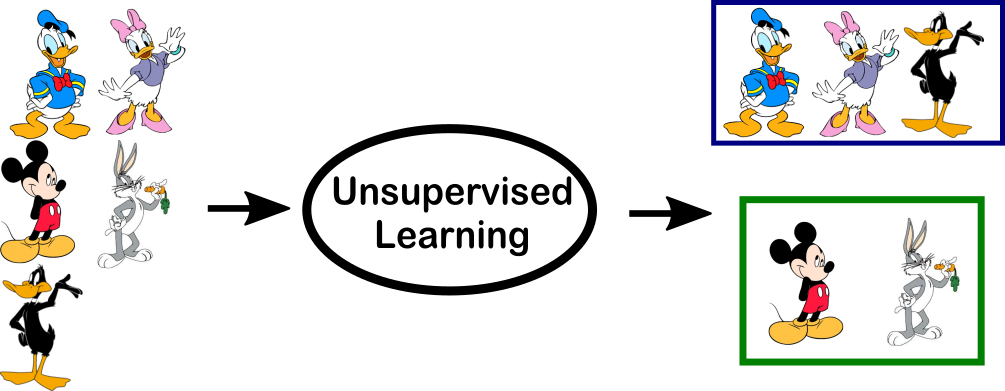
\includegraphics[width=150mm]{images/unsupervised.png}}

What do you do when your dataset doesn't have any labels? Unsupervised learning is a group of machine learning algorithms and approaches that work with what we call “no-ground-truth” data.\\
In unsupervised learning, an AI system is presented with unlabeled, uncategorized data and the system’s algorithms act on the data without prior training. The output is dependent upon the coded algorithms. Subjecting a system to unsupervised learning is one way of testing AI. With unsupervised learning, there is no feedback based on the prediction results.\\
The easiest way to understand what’s going on here is to think of a test. When you take tests in school, there are questions and answers; your grade is determined by how close your answers are to the actual ones (or the answer key). But imagine if there was no answer key, and there were only questions. How would you grade yourself?\\
Examples of unsupervised learning:\\
\textbf{Recommendations:} Music or items recommendation system\\
\textbf{Friends suggestions:} Suggestions on who you should follow on Instagram/Twitter/etc.

\section*{Reinforcement Learning}

Reinforcement Learning (RL) is a machine learning technique that enables an agent to learn in an interactive environment by trial and error using feedback from its own actions and experiences.\\
Though both supervised and reinforcement learning use mappings between input and output, unlike supervised learning where feedback provided to the agent is correct set of actions for performing a task, reinforcement learning uses rewards and punishments as signals for positive and negative behavior.\\
As compared to unsupervised learning, reinforcement learning is different in terms of goals. While the goal in unsupervised learning is to find similarities and differences between data points, in reinforcement learning the goal is to find a suitable action model that would maximize the total cumulative reward of the agent. The figure below represents the basic idea and elements involved in a reinforcement learning model.\\
\centerline{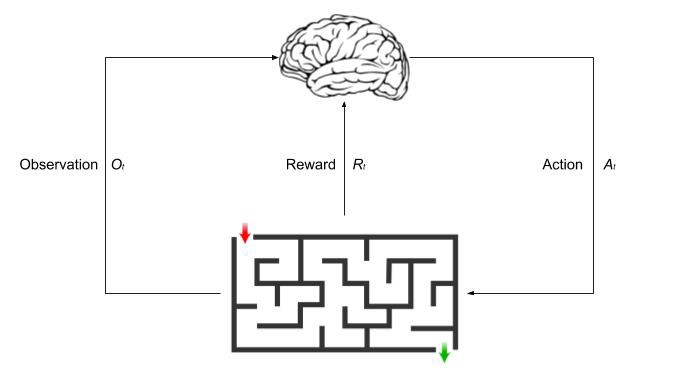
\includegraphics[width=150mm]{images/basic_ml.jpeg}}
Examples of reinforcement learning:\\
\textbf{Self-driving technology:}  Self-driving cars and trucks\\
\textbf{Autonomous Robots:}  Robots that can walk and perform multiple tasks on their own

\section*{The Future of Machine Learning}

\centerline{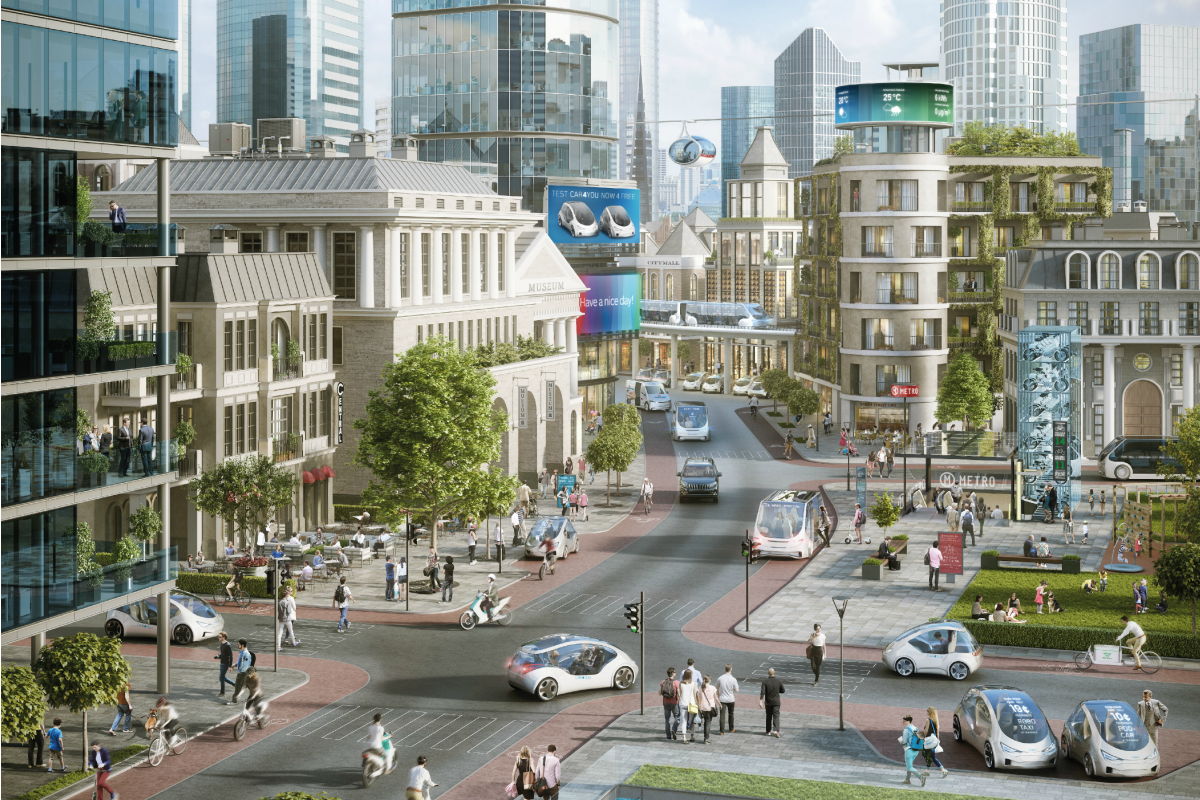
\includegraphics[width=150mm]{images/news-transport-july17-bosch3d.png}}

With no doubt, within 50 years, artificial intelligence will change everything we know about the world today. It is obvious why companies these days are trying to adopt this technology as quickly as possible into their businesses, and investors are betting their money into AI startups and research organizations.\\

However, most experts, regardless of whether they are optimistic or not, are expressing concern about these new tools and their long-term impact on the essential elements of being human. Many have shared deep worries, and many have also suggested pathways toward solutions.\\

\section*{More information!}

\begin{itemize}
    \item What is machine learning:
    \begin{itemize}
        \item \href{https://towardsdatascience.com/what-is-machine-learning-8c6871016736}{What is Machine Learning}
        \item \href{https://www.youtube.com/watch?v=ukzFI9rgwfU}{Machine Learning Basics | What Is Machine Learning? | Introduction To Machine
Learning | Simplilearn} (video)
    \end{itemize}
    \item Supervised Learning vs Unsupervised Learning:
\begin{itemize}    
        \item \href{https://towardsdatascience.com/unsupervised-learning-with-python-173c51dc7f03}{Unsupervised Learning with Python}
        \item \href{https://towardsdatascience.com/supervised-vs-unsupervised-learning-14f68e32ea8d}{Supervised vs Unsupervised Learning}
    \end{itemize}
    \item The future of Machine Learning:
    \begin{itemize}
        \item \href{https://medium.com/foursquare-direct/in-ten-years-the-future-of-ai-and-ml-fa68a527f378}{Ten years in the future of AI and ML}
        \item \href{https://www.forbes.com/sites/robertadams/2017/01/10/10-powerful-examples-of-artificial-intelligence-in-use-today/}{10 Powerful Examples of Artificial Intelligence in Use Today}
    \end{itemize}
\end{itemize}

%******************************************************************************%
%                                                                              %
%                               Ask your peers                                 %
%                                                                              %
%******************************************************************************%
\chapter{Ask Your Peers}

\begin{enumerate}
    \item Explain machine learning in simple terms.
    \item Explain the difference between supervised, unsupervised and reinforcement learning.
    \item Give 2 examples of a supervised machine learning algorithm, and briefly explain it.
    \item Give 2 examples of a unsupervised machine learning algorithm and briefly explain it.
\end{enumerate}

Read more on Google if you aren't able to answer these questions with confidence!


%******************************************************************************%
%                                                                              %
%                          Understanding Datasets                              %
%                                                                              %
%******************************************************************************%

\chapter{Understanding Datasets}

\centerline{
\includegraphics[width=75mm]{images/data_meme.jpg}}

\section*{Can you handle data?}

Machine learning depends heavily on data. It’s the most crucial aspect that makes algorithm training possible and explains why machine learning became so popular in recent years. But regardless of your actual terabytes of information and data science expertise, if you can’t make sense of data records, a machine will be nearly useless or perhaps even harmful.\\

The thing is, all datasets are flawed. That’s why data preparation is such an important step in the machine learning process. In a nutshell, data preparation is a set of procedures that help make your dataset more suitable for machine learning. In broader terms, the data prep also includes establishing the right data collection mechanism. And these procedures consume most of the time spent on machine learning. Sometimes it takes months before the first algorithm is built!\\

Think of data preparation as booking flights, hotels and packing your baggage for a trip. It’s very boring but when everything is ready and well prepared, the trip will be amazing.\\

\section*{Handling missing data}

\centerline{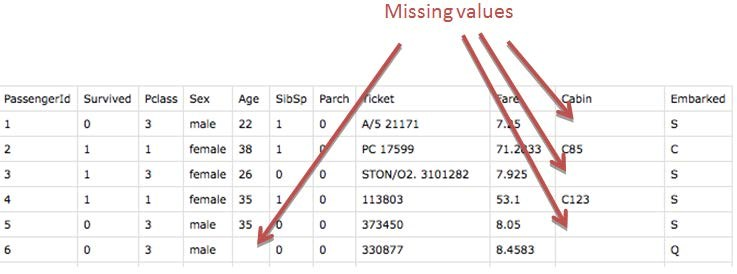
\includegraphics[width=100mm]{images/missing-values.png}}

The ideal datasets are the ones that are filled with data, but that’s not always the case in the real world scenario. You might have columns that are unfilled. So knowing how to handle missing values is greatly important to prepare a clean dataset.\\

Handling the missing values is one of the greatest challenges faced by analysts because making the right decision on how to handle it generates robust data models. Let us look at different ways of imputing the missing values.\\

\subsection*{Deleting rows}
We either delete a particular row if it has a null value for a particular feature and a particular column if it has more than 70-75\% of missing values. This method is advised only when there are enough samples in the data set.
\subsection*{Replacing with mean/median/mode}
This strategy can be applied on a feature which has numeric data like the age of a person or the ticket fare. We can calculate the mean, median or mode of the feature and replace it with the missing values. This is an approximation which can add variance to the data set. But the loss of the data can be negated by this method which yields better results compared to removal of rows and columns
\subsection*{Assigning An Unique Category}
A categorical feature will have a definite number of possibilities, such as gender, for example. Since they have a definite number of classes, we can assign another class for the missing values. This strategy will add more information to the dataset which will result in the change of variance.
\subsection*{Predicting The Missing Values}
Using the features which do not have missing values, we can predict the nulls with the help of a machine learning algorithm. This method may result in better accuracy unless a missing value is expected to have a very high variance

\section*{Categorical Data and Encoding}

Categorical data are variables that contain label values rather than numeric values. The number of possible values is often limited to a fixed set. Categorical variables are often called nominal.\\\\
Some examples include:\\
A “pet” variable with the values: “dog” and “cat“.\\
A “color” variable with the values: “red“, “green” and “blue“.\\
A “place” variable with the values: “first”, “second” and “third“. Each value represents a different category.\\\\

In my cases, you will see datasets with categorical data such as gender or nationality. But machine learning models are based on mathematics, you can intuitively understand that it will cause some problems if we keep the text here from the categorical variable in a machine learning equation. Many machine learning algorithms cannot operate on label data directly. They require all input variables and output variables to be numeric.\\

And that is why we need to encode the categorical variable (encode the text) into numbers. While there are many ways to do that, one of the most common methods is one hot encoding.\\

One hot encoding is a process by which categorical variables are converted into a form that could be provided to Machine learning algorithms to do a better job in prediction. This is where the integer encoded variable is removed and a new binary variable is added for each unique integer value.\\

\centerline{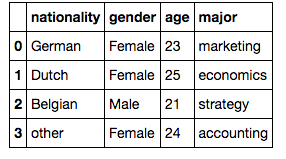
\includegraphics[width=75mm]{images/nationality_words.png}}
\centerline{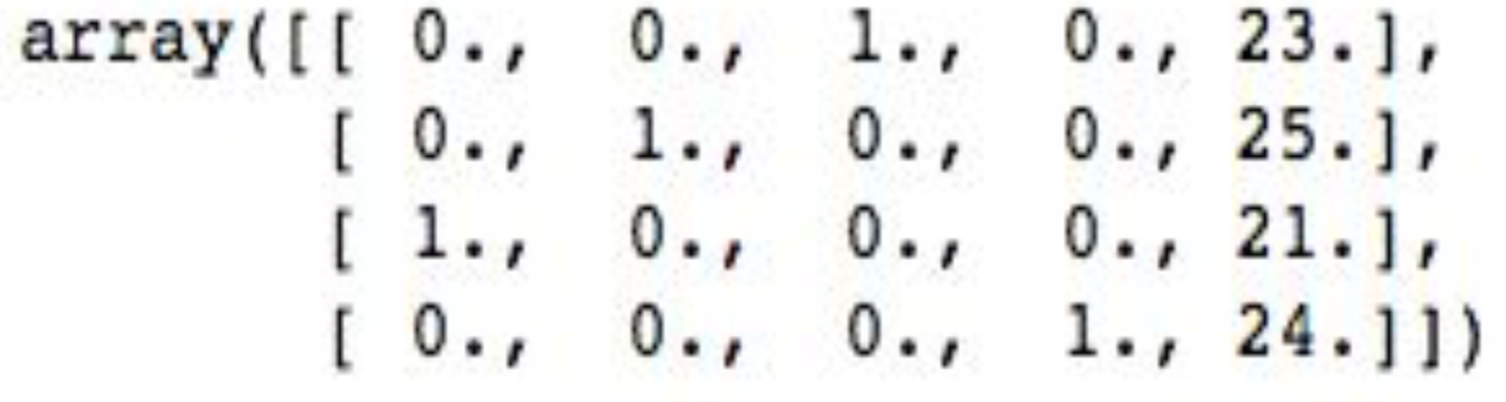
\includegraphics[width=75mm]{images/array_data.png}}
\centerline{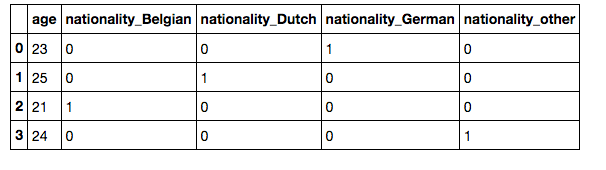
\includegraphics[width=150mm]{images/nationality_nums.png}}

\section*{Overfitting / Underfitting and Generalization}

One of the very common issues while developing Machine Learning systems is
overfitting.\\
Let me give you a classic example:\\
Suppose you have built a model to predict housing prices in the Bay Area. This is
typically a Linear Regression model.\\
Now, the Bay Area is big, big enough that you have an enormous amount of actual data, but of course, there are a lot more houses in the region than the amount of data you’ve used to train your model.\\
When you train your model, it tries its best to find out some kind of pattern in your training data while minimizing the error rate. But we only want our model to find a pattern. Not more than that.\\
Why? Because if your model just tries to go beyond finding patterns, it may memorize the training data. Look at the image below:\\

\centerline{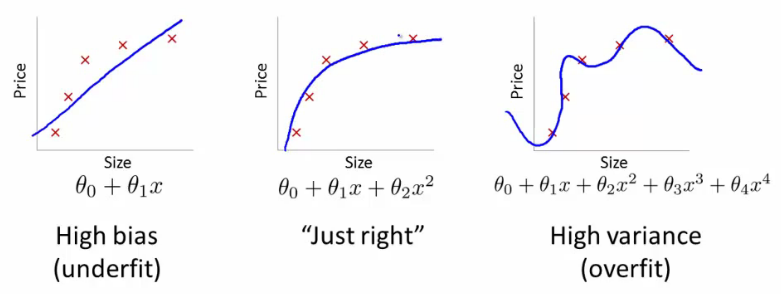
\includegraphics[width=150mm]{images/bias_variance_typed.png}}

In the leftmost graph, your model has not quite understood any pattern in your data. We call it underfitting - it fits the data worse than it should.\\
The middle one depicts a model which has found a just right pattern in the training data. This is quite reasonable.\\
The third one is a model where things are pretty much messed up.\\
In the third one, your model has found a pattern in the training set, but it has kind of memorized it! If you check out the training accuracy for this particular model, you will see that the accuracy is just 100\% with simply 0 error. But will this model outperform the middle one in newer examples? Discuss with your friends about it!\\
One word you will hear a lot in machine learning is called \textbf{“generalization”}. The meaning of generalization is - The ability of the learned model to fit an unseen instance. The goal of machine learning is to let the learned model fit unseen instance well. A model with strong generalization ability can fit the whole sample space well.\\
So the lesson here is this. To create good predictive models in machine learning that are capable of \textbf{generalizing}, one needs to know when to stop training the model so that it doesn't overfit. Just like a parent, sometimes a programmer needs to know when to kick their kid out of the house and have them go into the real world. Otherwise, they'll know everything about their parents' basement and yet be incapable of doing anything productive outside that small enclosure. :P\\

\section*{Data Splitting: Training Set and Test Set}

The fundamental goal of ML is to generalize beyond the data instances used to train models. We want to evaluate the model to estimate the quality of its pattern generalization for the data the model has not been trained on.\\

However, since future instances have unknown target values and we cannot check the accuracy of our predictions for future instances now, we need to use some of the data that we already know the answer for as a proxy for future data. Evaluating the model with the same data that was used for training is not useful, because it rewards models that can “remember” the training data, as opposed to generalizing from it.\\

A common strategy is to take all available labeled data, and split it into training and testing subsets, usually with a ratio of 70-80 percent for training and 20-30 percent for evaluation (testing).\\

\subsection*{Training set}
The actual dataset that we use to train the model. The model sees and learns from this data.
\subsection*{Test set}
The sample of data used to provide an unbiased evaluation of a final model fit on the training dataset.

\centerline{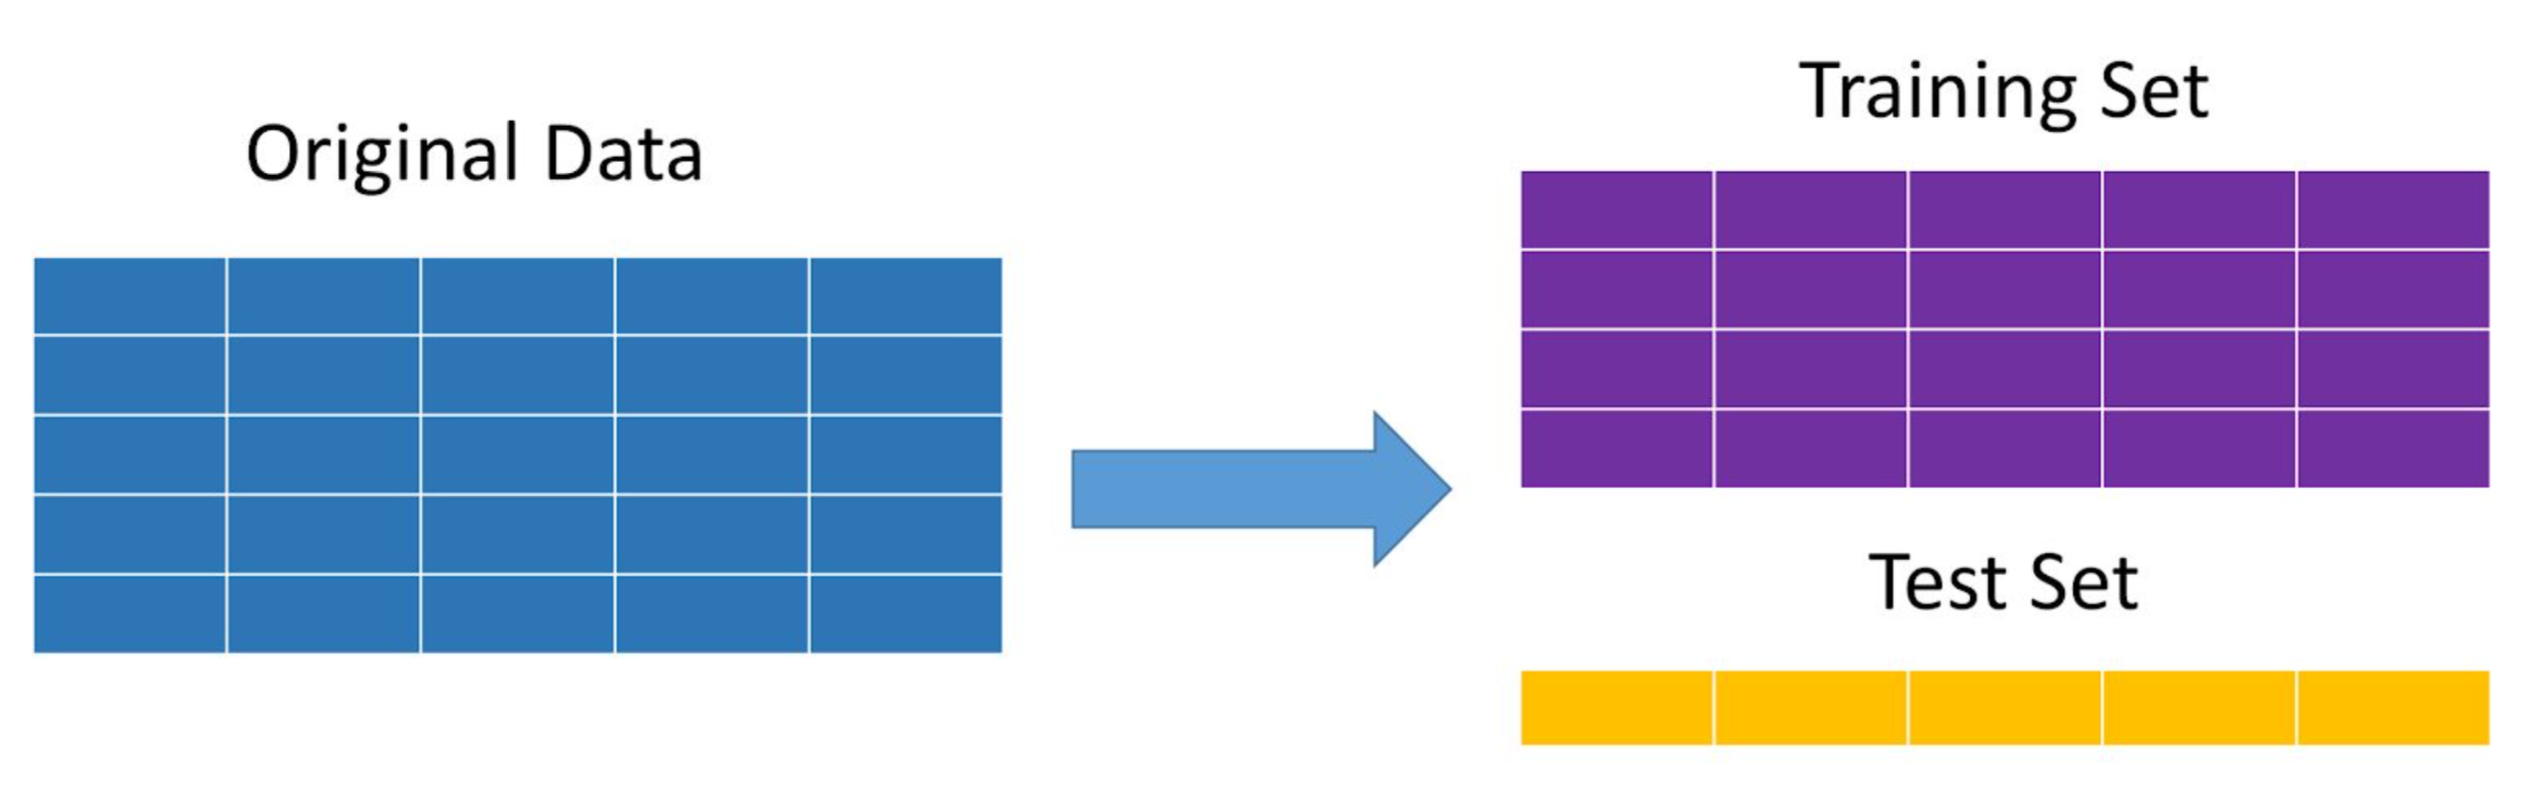
\includegraphics[width=150mm]{images/training_test.png}}

\section*{Feature scaling}

Most of the time, your dataset will contain features highly varying in magnitudes, units, and range. But since most of the machine learning algorithms use Euclidean distance between two data points in their computations, this is a problem.\\

If left alone, these algorithms only take in the magnitude of features neglecting the units. Let’s say you have two lengths, L1 = 250 cm and L2 = 2.5 m. We, humans, see that these two are identical lengths (L1 = L2), but most ML algorithms interpret this quite differently.\\

You see, the algorithm is going to give a lot more weight to L1, simply because it is expressed in a larger number, which, in turn, is going to have a much larger impact on the prediction than L2.\\

There are many different scaling algorithms. The most common one is the Standard Scaler. It assumes that your data follows a Gaussian distribution (Gaussian distribution is the same thing as Normal distribution).\\

The mean and the standard deviation are calculated for the feature and then the feature is scaled based on:
\[ (xi - mean(x)) / stdev(x) \]

The idea behind Standard Scaler is that it will transform your data, such that the distribution will have a mean value of 0 and a standard deviation of 1.\\

\centerline{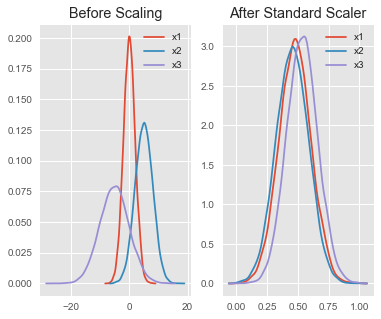
\includegraphics[width=150mm]{images/std_scale.png}}

\newpage

\section*{More information!}

\begin{itemize}
    \item Handling missing data:
    \begin{itemize}
        \item \href{https://www.analyticsindiamag.com/5-ways-handle-missing-values-machine-learning-datasets/}{5 Ways To Handle Missing Values In Machine Learning Datasets}
        \item \href{https://towardsdatascience.com/how-to-handle-missing-data-8646b18db0d4}{How to handle missing data}
    \end{itemize}
    \item Categorical Data and Encoding:
\begin{itemize}    
        \item \href{https://hackernoon.com/what-is-one-hot-encoding-why-and-when-do-you-have-to-use-it-e3c6186d008f}{What is One Hot Encoding? Why And When do you have to use it?}
        \item \href{https://towardsdatascience.com/encoding-categorical-features-21a2651a065c}{Encoding Categorical Features}
        \item \href{https://towardsdatascience.com/smarter-ways-to-encode-categorical-data-for-machine-learning-part-1-of-3-6dca2f71b159}{Smarter Ways to Encode Categorical Data for Machine Learning}
    \end{itemize}
    \item Overfitting/Underfitting and Generalization:
    \begin{itemize}
        \item \href{https://medium.com/greyatom/what-is-underfitting-and-overfitting-in-machine-learning-and-how-to-deal-with-it-6803a989c76}{What is underfitting and overfitting in machine learning and how to deal with it}
        \item \href{https://towardsdatascience.com/train-test-split-and-cross-validation-in-python-80b61beca4b6}{Train/Test Split and Cross-Validation in Python}
        \item \href{https://elitedatascience.com/overfitting-in-machine-learning}{Overfitting in Machine Learning: What It Is and How to Prevent It}
        \item \href{https://towardsdatascience.com/regularization-in-machine-learning-76441ddcf99a}{Regularization in Machine Learning}
    \end{itemize}
    \item Data Splitting: Training Set and Test Set:
    \begin{itemize}
            \item \href{https://medium.com/datadriveninvestor/what-are-training-validation-and-test-data-sets-in-machine-learning-d1dd1ab09bae}{What are training, validation, and test data sets in machine learning?}
            \item \href{https://towardsdatascience.com/train-validation-and-test-sets-72cb40cba9e7}{About Train, Validation and Test Sets in Machine Learning}
    \end{itemize}
    \item Feature scaling:
    \begin{itemize}
            \item \href{https://medium.com/@ian.dzindo01/feature-scaling-in-python-a59cc72147c1}{Feature Scaling in Python}
            \item \href{https://medium.com/greyatom/why-how-and-when-to-scale-your-features-4b30ab09db5e}{Why, How and When to Scale your Features}
    \end{itemize}
\end{itemize}

%******************************************************************************%
%                                                                              %
%                               Ask your peers                                 %
%                                                                              %
%******************************************************************************%
\chapter{Ask Your Peers}

\begin{enumerate}
    \item What are the ways to handle missing data? State 2 of them and their method.
    \item What is considered a categorical data and why do we need to encode them?
    \item Besides one hot encoding, state and explain 2 more encoding techniques
    \item What does it mean to overfit our model?
    \item What is the meaning of generalization in machine learning?
    \item What is a training set and test set? And what is the common splitting ratio?
    \item What is feature scaling and why do we need to do it?
    \item What are the feature scaling methods? State 2 more besides Standard Scalar.
\end{enumerate}

Read more on Google if you aren't able to answer these questions with confidence!

\end{document}